\documentclass[twoside,openright,a4paper,12pt]{report} %,draft,openright

\usepackage{polski}
\usepackage[utf8]{inputenc} 
\usepackage{gensymb}
\usepackage{epsf,graphicx}
\usepackage{subfigure}
\usepackage{latexsym,amssymb}
\usepackage{setspace,cite}
\usepackage{indentfirst}
\usepackage{mathtools}
\usepackage[justification=centering]{caption}
\usepackage{multirow}
\usepackage[figuresright]{rotating}
\usepackage{listings}

% for margins left, right top bottom
\usepackage{anysize}
\marginsize{3cm}{2.5cm}{2.5cm}{2.5cm}
%\let\origdoublepage\cleardoublepage    %%komenda wstawiająca czyste kartki
%\newcommand{\clearemptydoublepage}{%
%  \clearpage
%  {\pagestyle{empty}\origdoublepage}%
%}
%\let\cleardoublepage\clearemptydoublepage
\graphicspath{ {Resources/} }


%\usepackage{draft} %draft option - doesn't put full figures in -
            % useful when editing

%does the headers on the pages - keep in
\usepackage{fancyhdr}

%omitting any of these makes the thesis compile without the omitted
%chapter - good for editing single chapters.
%\includeonly{header,appendix}


\begin{document}

%Puts page numbering of preamble in roman and of main body of thesis in
%arabic. Also defines how chapters and sections are made
\pagenumbering{arabic}
\setcounter{page}{1} \pagestyle{fancy}
\renewcommand{\chaptermark}[1]{\markboth{\chaptername%
\ \thechapter:\,\ #1}{}}
\renewcommand{\sectionmark}[1]{\markright{\thesection\,\ #1}}

%DEFINES TITLE PAGE, and contains abstract, acknowledgements, etc.

%%%%%%%%%%%%%%%%%%%%%%%%%%%%%%%%%%%%%%%%%%%%%%%%%%%%%%%%%%%%%%%%%%%%%%%%%%%
% This is a sample header for a sample dissertation. Fill in the name,
% and the other information. LaTeX will work out the table of
% content, the list of figures and of tables for you.
%%%%%%%%%%%%%%%%%%%%%%%%%%%%%%%%%%%%%%%%%%%%%%%%%%%%%%%%%%%%%%%%%%%%%%%%%%%

\newpage
\thispagestyle{empty}




% ******* Title page *******
% **************************

\begin{onehalfspacing}
\begin{center}

\centering

\includegraphics[keepaspectratio,scale=0.1]{./figures/godlo.PNG} \\[.8cm]


{\fontsize{17}{17}\selectfont
\textsc{Politechnika Śląska \\[.3cm]
Wydział Automatyki, Elektroniki i Informatyki  \\[.3cm]
Kierunek Informatyka  \\[2.5cm]}
\textbf{Praca dyplomowa magisterska \\[1.7cm]}}



\large 
{Algorytm wyszukiwania z tabu do rozwiązywania problemu układania planu zajęć} \\[3.1cm]
% Jeśli tytuł pracy zajmuje 2 linijki, wartość [2.3cm] zamieniamy na [3.1cm], jeśli tylko jedną - na [3.9cm] i odwrotnie - zwiększając liczbę linijek o jedną (do czterech) zmieniamy na [1.5cm] itd.


\large
\begin{flushleft}
Autor: Michał Szluzy  \\
Kierujący pracą:  prof. dr hab. inż. Zbigniew Czech \\
\end{flushleft}

\vspace{2cm}
Gliwice, czerwiec 2017
\end{center}
\end{onehalfspacing}

\singlespacing
\newpage

\thispagestyle{empty}
\mbox{}


%ABSTRACT
\begin{abstract}
W niniejszej pracy został opisany proces przystosowania algorytmu wyszukiwania z tabu do rozwiązywania problemu układania planu zajęć. Aspektem badawczym pracy było zbadanie wpływu parametrów zaimplementowanego algorytmu na szybkość jego działania i otrzymane wyniki. Omówione zostały podstawy teoretyczne badanego problemu oraz trudności towarzyszące implementacji algorytmu jego rozwiązania. Testowanie algorytmu zostało przeprowadzone na danych rzeczywistych, a wyniki zaprezentowane na wykresach.
\end{abstract}
%END OF ABSTRACT

\setcounter{page}{4} 
\doublespacing
\mbox{}

%\pagestyle{empty}
%\pagenumbering{Roman}
%\setcounter{page}{0} \pagestyle{plain}


\tableofcontents

\listoffigures
%\listoftables

\newpage
\thispagestyle{empty}


%\pagestyle{fancy}



%sets up headers for lefthand and righthand pages. To alter, edit
%these lines and the chaptermark/sectionmark lines above
%\addtolength{\headheight}{3pt} \fancyhead{}
%\fancyhead[LE]{\sl\leftmark} \fancyhead[LO,RE]{\rm\thepage}
%\fancyhead[RO]{\sl\rightmark} \fancyfoot[C,L,E]{}
\pagenumbering{arabic}
\fancyhead[LE,RO]{\slshape \rightmark}
\fancyhead[LO,RE]{\slshape \leftmark}
\fancyfoot[C]{\thepage}


\setlength{\parskip}{1ex} %odstępy między akapitami
%\singlespacing
%\doublespacing
\onehalfspacing
\chapter{Wstęp}


Problem układania planu zajęć jest dobrze znany w środowiskach szkolnych i akademickich. Układanie planu to zajęcie żmudne oraz wymagające dużej spostrzegawczości i wyobraźni u osoby, która plan układa. Problem ten jest aktualny każdego roku, lub w przypadkach koniecznych np. przy zmianie liczby prowadzących, bądź zmienionej siatce zajęć. Układanie planu zajęć metodami tradycyjnymi pochłania dużo czasu i często kończy się niepowodzeniem. Jeżeli już uda się ułożyć plan, to często nie jest on najlepszy i nie spełnia oczekiwań uczniów bądź nauczycieli. Dlatego też badacze w wielu środowiskach na świecie rozważają problem układania planu zajęć i poszukują efektywnych algorytmów jego rozwiązania. W obecnych czasach mało która szkoła lub uczelnia nie wspomaga się przy tej czynności komputerem. Możliwość szybkiego utworzenia i ocenienia wielu planów lub uzyskanie wiedzy, czy dany plan jest możliwy do zrealizowania, to tylko niektóre zalety zastosowania do tego celu komputera. Najważniejszą zaletą jest możliwość skorzystania z algorytmów, które w krótkim czasie, np. 10 minut, ułożą plan zajęć zgodnie z podanymi założeniami.

Celem niniejszej pracy jest zbadanie możliwości zastosowania algorytmu wyszukiwania z tabu do problemu układania planu zajęć. Algorytm ten, rozwiązujący trudne problemy z wielu dziedzin życia, może być również zastosowany do rozwiązywania problemu układania planu zajęć. Praca oparta jest na materiałach źródłowych, w których do optymalizacji układania planu zajęć wykorzystano różne algorytmy heurystyczne. Korzystając z doświadczeń poprzedników, udało się uniknąć typowych błędów pojawiających się przy implementacji algorytmów rozwiązywania rozważanego problemu.

Aspektem badawczym pracy jest zbadanie wpływu parametrów zaimplementowanego algorytmu na szybkość jego działania i otrzymywane wyniki. Korzystając z dużej bazy danych testowych pochodzących z różnych szkół i uczelni na świecie dokonamy testowania algorytmu dla rzeczywistych problemów układania planu zajęć.

Praca, poza wstępem i zakończeniem, składa się z pięciu rozdziałów oraz jednego dodatku. Pierwszy rozdział poświęcony jest omówieniu algorytmu wyszukiwania z tabu. Przedstawiono w nim cechy algorytmów heurystycznych i metaheurystycznych oraz genezę algorytmu wyszukiwania z tabu. W rozdziale znaleźć można również omówienie podstawowej idei działania algorytmu oraz różnych jego wariantów. Zdefiniowano także podstawowe pojęcia związane z algorytmem, takie jak sąsiedztwo, kryterium aspiracji, dywersyfikacja, intensyfikacja, etc. Drugi rozdział formułuje problem układania planu zajęć. Zawiera formalizację problemu i omówienie ograniczeń związanych z planami zajęć. Przedstawiona jest również złożoność problemu układania planu zajęć w celu uzasadnienia potrzeby zastosowania algorytmów heurystycznych. Kolejny rozdział w całości poświęcony jest formatowi danych wejściowych, jakie są niezbędne do zaimplementowania algorytmu w celu poprawnego działania. Używany format danych jest wykorzystywany w problemie układania planu zajęć przez wielu badaczy na całym świecie. Opisanie formatu pozwala zrozumieć problemy, z jakimi trzeba się zmierzyć podczas implementowania algorytmu. Implementacja algorytmu oraz jego specyfikacja wewnętrzna i zewnętrzna zostały opisane w następnym rozdziale. Przedstawiono w nim funkcje wykorzystane w jej realizacji. Omówiono również wykorzystane podczas pracy narzędzia i środowiska. W ramach specyfikacji zewnętrznej przedstawiono opis interfejsu graficznego użytkownika oraz sposób korzystania z aplikacji. Ostatni rozdział opisuje proces testowania algorytmu. Omówiona została w nim specyfikacja środowiska testowego oraz zestaw danych wybrany do testowania. Wyniki działania aplikacji zostały zaprezentowane w postaci dwóch wygenerowanych planów zajęć wraz z oceną uzyskanych rozwiązań. Na końcu rozdziału zaprezentowano wpływ parametru długości listy tabu na wyniki działania algorytmu. Do pracy dołączono dodatek, w którym przedstawiono wybrane fragmenty kodu źródłowego.


\chapter{Algorytm wyszukiwania z tabu}
\section{Algorytmy heurystyczne i metaheurystyczne}
 Optymalizacja rozwiązań wykorzystywana jest w prawie każdym aspekcie życia. Podwyższanie jakości usług, obniżanie kosztów wyrobów, czy minimalizacja zużycia surowców to bardzo popularne zagadnienia optymalizacyjne. Medycyna, logistyka, ekonomia to przykłady dziedzin, w których optymalizacja znajduje swoje zastosowanie. 
 Optymalizacja to minimalizacja bądź maksymalizacja pewnej funkcji, zwanej często funkcją oceny, która określa jakość rozwiązania danego problemu. Znalezienie minimum lub maksimum wymaga więc wyznaczenia funkcji oceny dla każdego możliwego rozwiązania problemu i wyborze rozwiązania o najlepszej wartości funkcji oceny. Niestety często rozmiar zadania, dla którego szukamy optymalnego rozwiązania, jest tak duży, że sprawdzenie wszystkich rozwiązań, bądź zastosowanie algorytmu znajdującego najlepsze rozwiązanie nie jest możliwe ze względu na zbyt długi czas wykonania. Liczba operacji, które należy wykonać często rośnie wykładniczo wraz ze wzrostem rozmiaru problemu. Stwarza to możliwość zastosowania heurystyk.
 
 ,,Terminem heurystyka (z języka greckiego heurisko - znajduję) określa się sposób postępowania oparty na zdobytym doświadczeniu, wykorzystaniu istniejących faktów i reguł, w celu znalezienia odpowiedzi na postawione pytanie"\cite{Algorytmy:Widuch}. Algorytmy heurystyczne to takie algorytmy, które na podstawie przebiegu obliczeń i otrzymywanych wynikach, starają się znaleźć jak najlepsze rozwiązanie problemu, jednak zwykle nie jest to rozwiązanie optymalne (tj. najlepsze wśród wszystkich możliwych rozwiązań). W zamian za możliwość otrzymania nieco gorszego rozwiązania uzyskamy krótszy czas działania algorytmu. Algorytmy heurystyczne wykorzystywane są w przypadku, gdy dokładne algorytmy są z przyczyn technicznych zbyt kosztowne, lub gdy są nieznane (np. dla problemu przewidywania pogody). Często też używa się heurystyk by ,,nakierować'' gotowy algorytm na rozwiązanie optymalne, co w rezultacie skróci czas jego wykonania.
 
 Algorytmy heurystyczne możemy podzielić ze względu na sposób, w jaki generowane są nowe rozwiązania:
 \begin{itemize}
 	\item Algorytmy probabilistyczne - wykorzystują czynnik losowości; często kolejne rozwiązanie wybierane jest losowo z określonej puli rozwiązań. Może to doprowadzić do różnych wyników końcowych otrzymanych w kolejnych wykonaniach algorytmu.
 	\item Algorytmy deterministyczne - nie zawierają czynnika losowego. Otrzymywane rozwiązanie jest zawsze takie same, przy każdym wykonaniu algorytmu na takich samych danych wejściowych. 	
 \end{itemize}

W niektórych algorytmach wykorzystane są dwie heurystyki, nadrzędna i podrzędna. Pierwsza z nich steruje i uzupełnia działanie drugiej heurystyki. Takie podejście nazywane jest przez niektórych badaczy metaheurystykami \cite{Algorytmy:Widuch}. Inna definicja metaheurystyki to ,,procesy iteracje działające zgodnie z klasyczną metodą heurystyczną, wspomagane inteligentnie przez różne koncepcje eksplorowania i eksploatowania przestrzeni rozwiązań z użyciem technik uczących. Wspomaganie to ustrukturalnia informacje w celu sprawnego znalezienia rozwiązań bliskich optymalnemu" \cite{Metaheurystyki:Osman}. Po raz pierwszy termin metaheurystyki został użyty przez Freda Glovera w 1986 roku jako określenie algorytmów, które nie rozwiązują bezpośrednio żadnego problemu, lecz określają w jaki sposób budować algorytmy podrzędne w celu uzyskania rozwiązania \cite{Future:Glover}.

\section{Wyszukiwanie z tabu}

Przykładem algorytmu metaheurystycznego jest algorytm wyszukiwania z tabu. Algorytm ten został zaproponowany w 1977 r. kiedy to Fred Glover przedstawił pracę na temat wykorzystania pamięci krótkotrwałej i długotrwałej w przeszukiwaniu lokalnym. Pamięć krótkotrwała służyła do zapamiętywania ostatnich ,,ruchów'' algorytmu i była modyfikowana przez kolejne jego iteracje (pamiętane były wybrane wartości wykorzystywane przez algorytm w ostatnich iteracjach). Natomiast pamięć długotrwała miała na celu pamiętanie najbardziej atrakcyjnych rozwiązań przestrzeni poszukiwań. To właśnie w oparciu o tą zasadę, Glover zaproponował w 1986 r. algorytm \textit{Tabu Search}. Glover jest uznawany za autora algorytmu mimo tego, że w tym samym roku Michael Hansen opublikował pracę opisującą bardzo podobną heurystykę. Na przestrzeni lat algorytm został ulepszony i aktualnie dostępnych jest wiele jego różnych wersji, np. \textit{Probabilistic Tabu Search} lub \textit{Reactive Tabu Search}.

\subsection{Zasada działania algorytmu wyszukiwania z tabu}

Wyszukiwanie z tabu to metaheurystyka służąca do rozwiązywania problemów optymalizacji. Algorytm oparty na tej metaheurystyce dokonuje iteracyjnego przeszukiwania przestrzeni rozwiązań, z użyciem tzw. sąsiedztwa oraz na zapamiętuje ostatnio wykonane ruchy w celu uniknięcia ich powtarzania. Wywodzi się on bezpośrednio z metody przeszukiwania lokalnego, jednak jest od niej zdecydowanie skuteczniejszy dzięki możliwości ,,wychodzenia'' z minimów lokalnych. Podstawą tej możliwości jest zaakceptowanie gorszego aktualnego rozwiązania w celu uzyskania rozwiązania lepszego. Możliwe jest to dzięki uaktualnianiu danych tabu, czyli listy ruchów, które algorytm już wykonał, co zabezpiecza algorytm przed powrotem w obszary przestrzeni rozwiązań już przeszukane. Obecność ruchów na liście tabu jest tymczasowa, co w konsekwencji blokuje dany ruch przez określoną liczbę iteracji. Możliwe jest złamanie tej zasady, ale tylko wtedy, gdy ruch spełnia tzw. kryterium aspiracji. Warunkiem zakończenia działania algorytmu jest najczęściej wykonanie określonej liczba iteracji lub osiągnięcie satysfakcjonującego rozwiązania. Możliwe jest również monitorowanie aktualnego wyniku i, jeżeli nie ulega on poprawie przez określoną liczbę iteracji, zatrzymanie wykonania algorytmu. Pseudokod działania algorytmu przedstawiony został na rysunku 2.1.

\begin{figure}
	\centering
	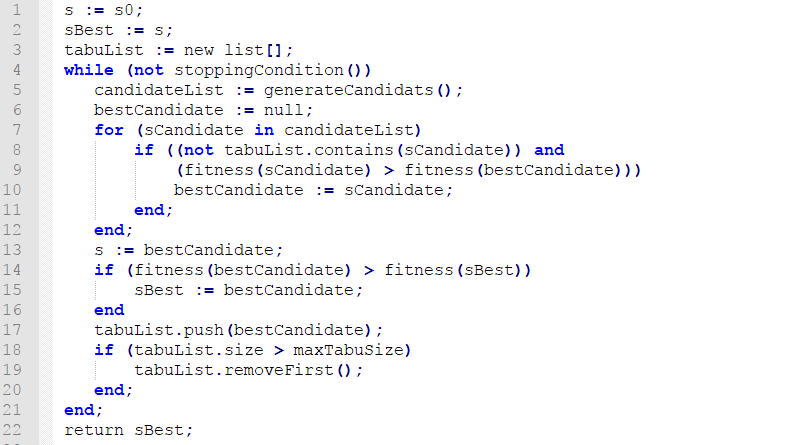
\includegraphics{PseudokodTabu}
	\caption{Pseudokod algorytmu Tabu search}
	\label{fig: AlgorytmTabu}
\end{figure}

\subsection{Sąsiedztwo rozwiązania}

Najważniejszym czynnikiem, od którego zależy sukces algorytmu jest poprawnie zdefiniowane sąsiedztwo, które będzie przeszukiwane w danej iteracji. Do sąsiedztwa powinny należeć rozwiązania różniące się w sposób nieznaczny od rozwiązania bieżącego. Jednak sąsiedztwo powinno umożliwiać algorytmowi przejście w każdy obszar przestrzeni rozwiązań. Sposób w jaki definiowane jest sąsiedztwo zależy od danego problemu i typu jego rozwiązań. Rozwiązania problemu mogą być reprezentowane np. przez wektory binarne, wektory liczb rzeczywistych, czy dowolne permutacje elementów zadanych zbiorów. Jeżeli na przykład rozwiązaniem będzie permutacja pewnego zbioru \textit{n} elementowego, to sąsiedztwem możemy określić jedno z trzech typów przejść (ruchów) między permutacjami:

\begin{itemize}
	\item wstaw(x, y) - wstawienie elementu y na pozycję x (permutacje z powtórzeniami),
	\item zamień(x, y) - zamiana elementów na pozycjach x i y,
	\item odwróć(x, y) - odwrócenie kolejności występowania elementów, począwszy od elementu o indeksie x, aż do elementu na pozycji y.
\end{itemize}

Sąsiedztwem danej permutacji będzie więc każda inna permutacja uzyskana za pomocą, wybranego na początku, sposobu modyfikacji bieżącej permutacji. Dzięki tak zdefiniowanemu sąsiedztwu możliwe jest łatwe zidentyfikowanie ruchu za pomocą pary indeksów (x, y). Para ta zostanie zapisana na liście tabu, a ruch ten będzie zablokowany przez następne iteracje.

Może się jednak okazać, że generowane sąsiedztwa są zbyt duże, by każdorazowo przeszukiwać je w całości. Stosowane jest wtedy zawężanie sąsiedztwa. Jednym ze sposobów zawężania jest losowy dobór sąsiedztwa. Wprowadza to element probabilistyczny do algorytmu, co zmniejsza prawdopodobieństwo powstania niepożądanych cykli. Jednak przy takim podejściu możemy pominąć obszary przestrzeni rozwiązań, w których znajduje się rozwiązanie optymalne.

\subsection{Kryteria aspiracji}

Może się zdarzyć, że zablokowanie pewnych ruchów doprowadzi do stagnacji procesu przeszukiwania lub całkowicie zablokuje kolejny ruch (np. w sytuacji, gdy wszystkie możliwe ruchy są na liście tabu). Jest to możliwe, ponieważ algorytm przechowuje tylko atrybuty rozwiązań, a nie całe rozwiązania. Kryterium aspiracji umożliwia zapobieganiu takiej sytuacji.
Spełnienie kryterium aspiracji pozwala na złamanie zakazu tabu, czyli wykonanie ruchu, który znajduje się na liście ostatnio wykonanych. Najpopularniejszym i najprostszym kryterium aspiracji jest uzyskanie najlepszego, nieznanego jak dotąd, wyniku. Musi być ono lepsze od aktualnie najlepszego w celu uniknięcia zapętleń. Jednak większość kryteriów aspiracji jest bardziej skomplikowana i opiera się na wyspecjalizowanym przewidywaniu możliwości powstania cyklu po wykonaniu określonego ruchu.

\subsection{Dywersyfikacji i intensyfikacja}

Ważnym aspektem algorytmu wyszukiwania z tabu jest pamięć długoterminowa. Służy ona do przechowywania danych o wykonanych już iteracjach i do budowania statystyk. Dzięki tym statystykom można modyfikować strategię poszukiwania. Głównym celem takich modyfikacji może być spełnienie jednego z dwóch kryteriów:
\begin{itemize}
	\item Intensyfikacja - jeżeli według statystyki, w danym obszarze znajduje się dużo dobrych rozwiązań to algorytm zagęści obszar poszukiwań. Dzięki temu istnieje szansa na znalezienie jeszcze lepszego rozwiązania w danym obszarze.
	\item Dywersyfikacja - jest to powiększenie obszaru poszukiwań. Najczęściej stosowanym sposobem jest nakładanie kary na ruchy, które powtarzają się w perspektywie dłuższego czasu. Efektem tego jest ,,przeniesienie" algorytmu w inne rejony poszukiwań, co zmniejsza szanse na pominięcie najlepszych rozwiązań.
\end{itemize}
Wykorzystanie intensyfikacji i dywersyfikacji w znaczniej mierze poprawia efektywność algorytmu, dlatego kryteria te są wykorzystywane w większości nowych wersji algorytmu \textit{Tabu Search}.





\chapter{Problem układania planu zajęć}
\section{Sformułowanie problemu}
Problem układania planu zajęć można sformułować następująco. Dana jest lista określonych wydarzeń, dostepnych okien czasowych i zasobów. Należy przyporządkować wydarzeniom okna czasowe oraz zasoby w taki sposób, by spełnić przyjęte założenia (rysunek 3.1). W formułowanym problemie:
\begin{itemize}
	\item wydarzeniami są poszczególne lekcje odbywające się w ciągu jednego tygodnia,
	\item dostępnymi oknami czasowymi są godziny w których mogą odbywać się zajęcia (np. od poniedziałku do piątku w godzinach między 8:00 a 18:00),
	\item zasoby to dostępne sale lekcyjne, nauczyciele prowadzący zajęcia, grupy uczniów itp.
\end{itemize}


\begin{figure}
	\centering
	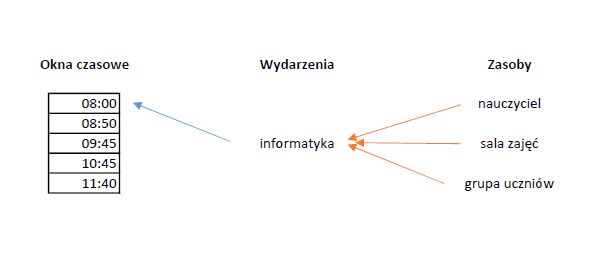
\includegraphics{podzialzasobow}
	\caption{Ilustracja problemu układania planu zajęć}
	\label{fig: podzialzasobow}
\end{figure}

Układanie planu zajęć wymaga spełnienia określonych ograniczeń. Mianowicie nie można wypełnić dostepnych okien czasowych według z góry przyjętej kolejności, ponieważ jest prawdopodobne, że pojawią się konflikty i plan zajęć nie będzie możliwy do zrealizowania. Aby tego uniknąć trzeba spełnić tzw. ograniczenia twarde, czyli takie, które zawsze muszą zostać spełnione, by plan mógł być możliwy do zrealizowania. Istnieją również ograniczenia miękkie, które określają jakość ułożonego planu. Ograniczenia te nie muszą zostać spełnione, ale algorytm układania planu zajęć powinien brać je pod uwagę.

\newpage
Przykłady ograniczeń:
\begin{itemize}
	\item twarde:
	\begin{itemize}
		\item zasób nie może być wykorzystany w dwóch miejscach w tym samym czasie (np. dany nauczyciel nie może prowadzić jednocześnie zajęć w dwóch różnych salach),
		\item nie występują zajęcia, które nie zostały przypisane do okien czasowych w ułożonym planie.
	\end{itemize}
	\item miękkie:
	\begin{itemize}
		\item brak dłuższych przerw między zajęciami dla uczniów,
		\item odpowiednie przerwy między zajęciami (np. 15 - lub 20 - minutowe),
		\item liczba dni roboczych, w których nauczyciele prowadzą zajęcia, powinna być minimalizowana,
		\item brak bloków zajęć danego typu (np. dana grupa uczniów nie powinna mieć kolejno czterech lekcji matematyki).
	\end{itemize}
\end{itemize}

%Niepodzielność zasobów oznacza, że jeden nauczyciel nie może być w dwóch miejscach jednocześnie, więc może prowadzić tylko jedne zajęcia w danym oknie czasowym, w jednej sali nie mogą się odbywać w tym samym czasie różne zajęcia, a dla danej grupy lekcje nie mają prawa się nakładać. Naruszenie tego ograniczenia było by fizycznie nie możliwe. 
%Obowiązek przypisania zajęć do jakichś okien czasowych oznacza, że na planie końcowym muszą się znaleźć wszystkie lekcje przewidziane w siatce zajęć dla danej grupy. Jest to podstawowe założenie bez którego układanie planu traci swój sens.
Często jednak dla wyjściowej siatki zajęć spełnienie wymagań twardych jest niemożliwe. Wynika to najczęściej z za małej liczby zasobów (za mało nauczycieli mogących prowadzić jeden przedmiot lub za mało sal). W algorytmach szuka się wtedy planu z najmniejszą liczbą niespełnionych wymagań, które są usuwane ręcznie przez szukanie określonych kompromisów (np. dołożenie okna czasowego, zatrudnienie dodatkowego nauczyciela, zaplanowanie zajęć tego samego typu dla dwóch mniejszych grup w jednej sali).

Ograniczenia miękkie to w istocie życzenia nauczycieli i uczniów co do tego jak  plan powinien wyglądać. Niespełnienie tych ograniczeń wpływa na końcową ocenę planu zajęć, niespelnione ograniczenia mogą mieć określone wagi w zależności od ich istotności. Niektóre plany zajęć układane są ze szczególnym uwzględnieniem uczniów (mała liczba okienek, równomierne rozłożenie zajęć, brak bloków zajęć tego samego typu, odpowiednia przerwa między zajęciami), a niektóre z uwzględnieniem potrzeb prowadzących (zajęcia skumulowane w ciągu dwóch dni tygodnia by umożliwić prace w innej szkole). Założenia te z reguły precyjzuje osoba uruchomiająca wykonanie planu przez odpowiednie skonfigurowanie parametrów algorytmu i zdefiniowanie funkcji oceny wygenerowanego planu.

Funkcja oceny planu zajęć z reguły przewiduje nakładanie punktów karnych za niespełnienie określonych ograniczeń. Każde ograniczenie ma ustaloną liczbę punktów karnych, przy czym ograniczenia twarde powinny mieć dużo większą wagę od ograniczeń miękkich. Im więcej punktów karnych ma plan tym jest gorszy. To właśnie na podstawie funkcji oceny planu większość algorytmów starta się ułożyć jak najlepszy plan zajęć.

\section {Rozmiar problemu}

By dobrze zrozumieć potrzebę używania algorytmów heurystycznych przy wyszukiwaniu najlepszego planu zajęć warto przybliżyć pojęcie skali problemu. W tym celu przedstawimy przykład planu zajęć dla amerykańskiej szkoły średniego rozmiaru. W przykładzie tym, każde ze zdarzeń ma przyporządkowane wcześniej zasoby. Przykład ten zawiera:

\begin{itemize}
	\item okna czasowe - 40,
	\item nauczyciele - 27,
	\item sale - 30,
	\item grupy uczniów - 24,
	\item zdarzenia - 832,
	\item ograniczenia - 4.
\end{itemize}

Dostępnych jest 40 okien czasowych, które rozłożone na pięć dni zajęć w tygodniu dają osiem godzin zajęć dziennie. Jednocześnie odbywać się mogą 24 zajęcia. Liczba ta wynika z niepodzielności zasobów i jest minimalną liczbą spośród liczby nauczycieli, sal i grup uczniów. Maksymalna liczba zdarzeń, które mogą się odbywać w danym tygodniu wynosi więc:
\[ 40 \cdot 24 = 960, \]
\[ 960 > 832. \]
Maksymalna liczba zdarzeń jest większa od liczby zdarzeń zawartych w siatce zajęć podanego przykładu, więc realizacja  planu zajęć zgodnego z powyższą specyfikacją zasobów jest możliwa.

Na jedną grupę uczniów przypada około 35 zdarzeń (832/24), które powinny być rozłożone na 40 okien czasowych. Uwzględniając możliwość wystąpienia okienek w trakcie zajęć, mamy więc 40-wyrazowy ciąg zdarzeń. Liczba możliwości, w które można te zajęcia rozłożyć, określa liczba permutacji 40!, która wynosi:
\[40! = 815915283247897734345611269596115894272000000000\]
Jest to 48 cyfrowa liczba możliwości rozłożenia zajęć w oknach czasowych dla jednej grupy. Liczbę tę trzeba pomnożyć przez liczbę grup.

Liczba możliwości może być jeszcze większa, jeżeli uwzględnimy to, że każde zajęcia mogą mieć przypisanego dowolnego nauczyciela z grupy osób uprawnionych do prowadzenia przedmiotu. Również sale zajęć mogą być różne dla danego wydarzenia. By zmniejszyć tę liczbę możliwości, odpowiednio modyfikuje się dane wejściowe. Każde zajęcia (zdarzenia) w danych wejściowych, mogą mieć przypisane na stałe zasoby takie jak sala, grupa i nauczyciel. Szukaną niewiadomą jest wtedy tylko termin odbywania się zajęć. Dzięki temu przestrzeń możliwych rozwiązań dla algorytmu układania planu zajęć zmniejsza się. Dodatkowo przypadek, w którym każde zajęcia mają wcześniej przypisanego prowadzącego, ma odzwierciedlenie w potrzebach współczesnych szkół, gdzie wyspecjalizowana kadra zatrudniana jest często w niepełnym wymiarze godzin, przez to może być przydzielona tylko do wybranej ilości zajęć.

Podejście, w którym zasoby, takie jak sala i nauczyciel, są przypisane z góry do zdarzeń, umożliwia szybsze działanie algorytmu. Jednak trzeba pamiętać, że ma to również wpływ na wynik końcowy. Może się zdarzyć przypadek, w który nie istnieje możliwość ułożenia optymalnego planu dla danych wejściowych, a wystarczyło by zamienić nauczyciela przypisanego do jednych zajęć, z innym nauczycielem tego samego przedmiotu, by odblokować nowe możliwości. Jednak z uwagi na czas działania algorytmu, jak i na dostępne dane testowe, zdecydowano się wybrać wariant, w którym do algorytmu przekazywane są zdarzenia z przypisanymi nauczycielami, salami oraz grupami, a algorytm wyszukuje tylko odpowiednie okna czasowe dla podanych zdarzeń.

\chapter{Format danych wejściowych}

Problem rozwiązywania planu zajęć jest zagadnieniem popularnym w świecie naukowym. Dostępnych jest wiele rozwiązań i ciągle powstają nowe. Jednak, by móc porównać ze sobą dwa różne algorytmy, konieczne jest operowanie na tych samych danych testowych. Z tego powodu naukowcy uzgodnili wspólny format danych wejściowych o nazwie XHSTT i stworzyli bazę danych wraz z przykładowymi rozwiązaniami \cite{Database}. Dane te zapisane są z wykorzystaniem języka XML. Format XHSTT ma duży stopień skomplikowania, dlatego postanowiono poświęcić cały rozdział na jego opisanie \cite{XHSTT}. 

\section{Budowa archiwum}

Archiwum jest kolekcją instancji zawierających dane dla problemu układania planu zajęć, razem z potencjalnymi grupami rozwiązaniami. Każda grupa rozwiązań zawiera rozwiązania dla jednej instancji z archiwum. Ogólny szablon dokumentu przedstawiono na rysunku 4.1. 

\begin{figure}
	\centering
	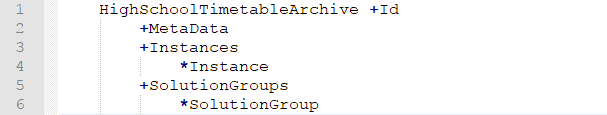
\includegraphics {szablonXHSTT}
	\caption{Szablon archiwum XHSTT.}
	\label{fig: szablonXhstt}
\end{figure}

W tej notacji, słowa znajdujące się w tej samej linii oznaczają, że pierwsze  słowo jest nazwą kategorii, a kolejne słowa to jej atrybuty. Słowa umieszczone poniżej w zagłębieniach to nazwy podkategorii. Znak + przed nazwą oznacza, że kategoria lub atrybut jest czymś opcjonalnym. Znak * oznacza, że dana kategoria może wystąpić zero lub więcej razy. Przykład w formacie XML zaprezentowano na rysunku 4.2.

\begin{figure}
	\centering
	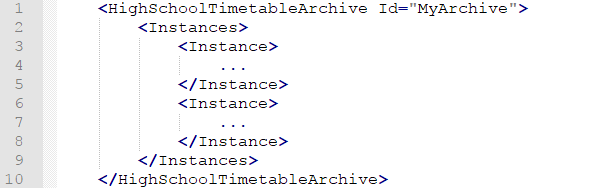
\includegraphics {szablonXHSTTprzyklad}
	\caption{Przykład archiwum w języku XML.}
	\label{fig: Xhsttprzyklad}
\end{figure}

Opcjonalna kategoria \textit{Metadata} zawiera podstawowe informacje na temat archiwum, takie jak: nazwa, autor, data powstania, opis oraz uwagi.

\section{Instancje}

Instancja jest to pojedynczy zestaw danych dla danego problemu układania planu zajęć, najczęściej dla pojedynczej szkoły i konkretnego roku (lub semestru). Składnie instancji zaprezentowano na rysunku 4.3. Wiele kategorii posiada atrybut \textit{Id}, który służy do odnoszenia się do danej kategorii w dalszej części archiwum.

\begin{figure}
	\centering
	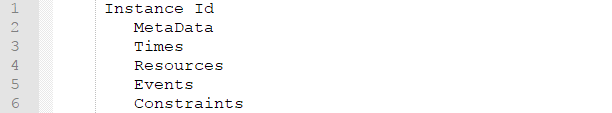
\includegraphics {skladniaSzablon}
	\caption{Szablon pojedynczej instancji.}
	\label{fig: skladniaSzablon}
\end{figure}

\section{Okna czasowe}

Format XHSTT wspiera tylko prosty model czasu, gdzie czas podzielony jest na równe interwały zwane oknami czasowymi. Kategoria \textit{Times} służy do definiowania tych okien. Podkategoria \textit{TimeGroups} definiuje różne grupy czasowe takie jak dni, tygodnie oraz okresy w ciągu dnia. Podkategoria \textit{Time} zawiera definicje okna czasowego, gdzie każde okno oprócz nazwy może mieć przypisany konkretny tydzień, dzień i inne grupy czasowe. Składnia kategorii \textit{Times} wraz z podkategoriami znajduje się na rysunku 4.4. Przykład w języku XML znajduje się na rysunku 4.5. Przedstawia on czwarte okno czasowe w poniedziałek.

\begin{figure}
	\centering
	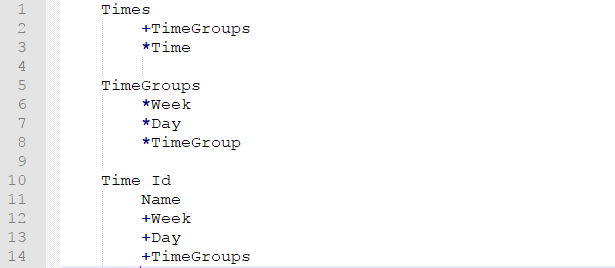
\includegraphics {skladniaTimes}
	\caption{Składnia kategorii: \textit{Times}.}
	\label{fig: skladniaTimes}
\end{figure}

\begin{figure}
	\centering
	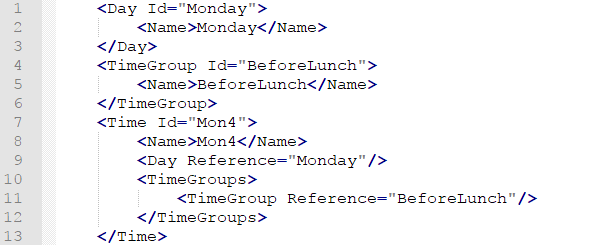
\includegraphics {timesPrzyklad}
	\caption{Przykład deklaracji czwartego okna czasowego w poniedziałek.}
	\label{fig: timesPrzyklad}
\end{figure}

\section{Zasoby}

Zasoby są to wszystkie elementy przypisane do zdarzeń. Do zasobów najczęściej zaliczamy nauczycieli, sale i grupy uczniów, ale format XHSTT dopuszcza dowolne definiowanie zasobów. W skład kategorii \textit{Resources} wchodzą również grupy i typy zasobów. Typ zasobów to np: nauczyciel, sala, grupa. Grupy zasobów gromadzą zasoby jednego typu np: nauczyciele języka polskiego. Składnia kategorii \textit{Resources} zaprezentowana jest na rysunku 4.6, na rysunku 4.7 zaprezentowano przykładową deklarację sali komputerowej.

\begin{figure}
	\centering
	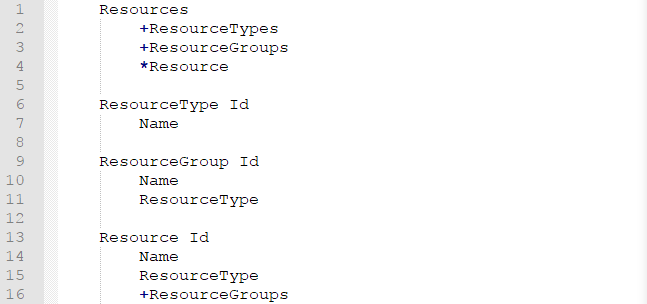
\includegraphics {resourcesSkladnia}
	\caption{Składnia kategorii: \textit{Resources}.}
	\label{fig: resourcesSkladnia}
\end{figure}

\begin{figure}
	\centering
	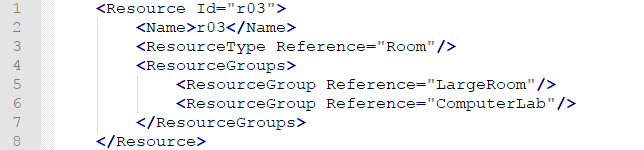
\includegraphics {resourcesPrzyklad}
	\caption{Przykład deklaracji zasobu jako sali komputerowej.}
	\label{fig: resourcesPrzyklad}
\end{figure}

\section{Zdarzenia}

Zdarzenia określone jest jako spotkanie pomiędzy zasobami, czyli w uproszczeniu są to zajęcia odbywające się w konkretnej sali, z konkretnym nauczycielem i grupą studentów. Przed zdarzeniami zdefiniowane mogą być ich grupy, takie jak np. zajęcia z kursu języka obcego. Same zdarzenia zawierają atrybuty określające ich czas trwania oraz termin odbycia się zajęć. Termin odbywania zajęć może być przypisany wcześniej lub może być pozostawiony pusty, w celu przypisania go przez algorytm układający plan zajęć. Dodatkowo zdarzenia posiadają parametr określający kolor zajęć wyświetlany na ułożonym planie. Składnia kategorii \textit{Events} zaprezentowana jest na rysunku 4.8, na rysunku 4.9 zaprezentowano przykładową deklarację zajęć z języka angielskiego.

\begin{figure}
	\centering
	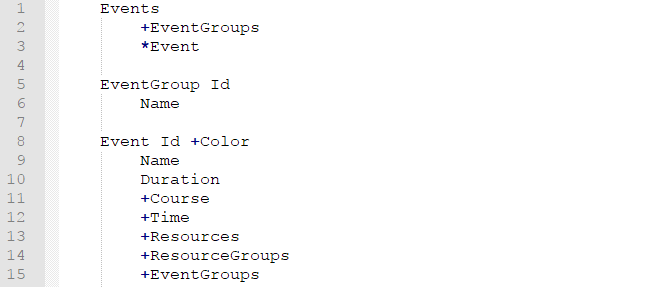
\includegraphics {eventsSkladnia}
	\caption{Składnia kategorii: \textit{Events}.}
	\label{fig: eventsSkladniakladnia}
\end{figure}

\begin{figure}
	\centering
	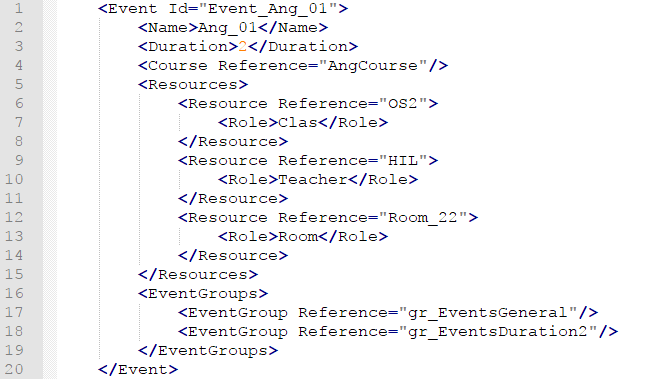
\includegraphics {eventsPrzyklad}
	\caption{Przykład deklaracji zajęć języka angielskiego.}
	\label{fig: eventsPrzyklad}
\end{figure}

\section{Ograniczenia}

Format XHSTT pozwala definiować wiele ograniczeń planu zajęć. Wszystkie one opisane są szczegółowo na stronie internetowej \cite{ograniczenia}. W pracy zostały opisane tylko te, które są uwzględnione w implementacji. Ogólna składnia ograniczenia przedstawiona jest na rysunku 4.10. Każde z ograniczeń ma zdefiniowaną swoją wagę oraz sposób wyliczania funkcji kosztu (liniowa, kwadratowa). Każde ograniczenie jest rozdzielone na ograniczenie twarde lub miękkie poprzez parametr \textit{Required}.

\begin{figure}
	\centering
	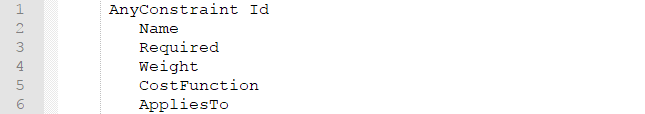
\includegraphics {ograniczeniaSkladnia}
	\caption{Składnia kategorii: \textit{Constraints}.}
	\label{fig: ograniczeniaSkladnia}
\end{figure}

\subsection{Przypisany czas}

Ograniczenie \textit{Assign time constraints} określa, że każde zdarzenie musi mieć przypisany czas oraz definiuje koszt złamania tego ograniczenia. Może być przypisane do wszystkich wydarzeń lub tylko do wybranych grup. Przykład przedstawiono na rysunku 4.11.

\subsection{Unikanie konfliktów}

Ograniczenie \textit{Avoid clashes constraints} określa, czy dane zasoby mogą być podzielone. To znaczy, czy nie są przypisane do dwóch lub więcej zdarzeń odbywających się w tym samym czasie. Jest to ograniczenie stosowane powszechnie, jednak mogą zdarzyć się przypadki, że układający dopuszcza odbywanie się dwóch zajęć w jednej sali jednocześnie (np. zajęcia wychowania fizycznego).

\subsection{Podział zdarzeń}

Ograniczenie \textit{Split events constraints} określa, czy zdarzenia o długości dłuższej niż jeden mogą zostać podzielone i rozłożone na kilka dni. Ograniczenie to pozwala nam definiować minimalne i maksymalne długości bloków jednego zdarzenia.

\subsection{Limit bezczynności}

Ograniczenie \textit{Limit idle times constraints} określa, czy mogą występować i jak długie są dopuszczalne przerwy między zajęciami. Określają, czy pomiędzy dwoma zajęciami jednego dnia, może wystąpić jedno lub więcej nieprzypisanych okien czasowych.

\begin{figure}
	\centering
	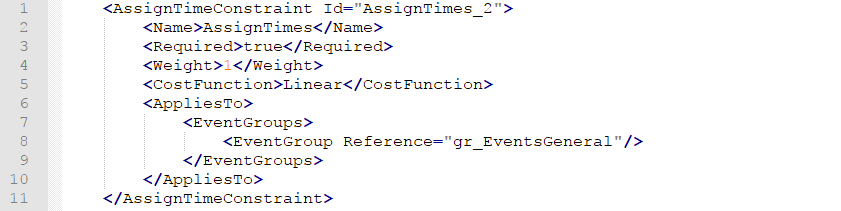
\includegraphics {ograniczeniaPrzyklad}
	\caption{Przykład ograniczenia: \textit{Assign time constraints}.}
	\label{fig: ograniczeniaPrzyklad}
\end{figure}
\chapter{Program układania planu zajęć}

Implementacja algorytmu została napisana w języku C\#. Język ten został wybrany z uwagi na dużą liczbę bezpłatnych bibliotek oraz możliwość dostępu do bardzo dobrej dokumentacji technicznej. Nie bez znaczenia był także fakt dużej popularności języka, co skutkuje większymi możliwościami uzyskania pomocy na forach programistycznych.

\section{Użyte narzędzia}

Podczas implementowania algorytmu wyszukiwania z tabu użyto następujących narzędzi:

\begin{itemize}
	\item Język programowania C\# - jest to obiektowy język programowania, którego początki sięgają roku 1998. Został zaprojektowany dla firmy Microsoft przez Andersa Hejlsberga. Program napisany w tym języku jest kompilowany do języka \textit{Common Intermediate Language} (CIL), który jest wykonywany w środowisku \textit{.NET Framework}. Jest to język prosty, o dużych możliwościach i wielu cechach wspólnych z językami programowania C++ oraz Java \cite{Csharp}. 
	
	\item Biblioteka Linq - Language-Integrated Query (LINQ) pozwala odczytywać dane pochodzące z różnych źródeł w postaci obiektów. Biblioteka udostępnia funkcje filtrujące i wyszukujące, które odpowiednio użyte w znacznej mierze przyspieszają działanie programu. W implementacji algorytmu, którego dotyczy praca, zapytania Linq ułatwiają komunikację z bazą danych oraz czytanie dokumentów XML.
	
	\item Windows Forms - interfejs programowania graficznych aplikacji należący do środowiska \textit{.NET Framework}. Służy do tworzenia aplikacji z graficznym interfejsem użytkownika, umożliwiająca obsługę zdarzeń napływających od użytkownika. Obecnie interfejs wypierany jest przez interfejs Windows Presentation Foundation  (\textit{WPF}). Jednak mimo tego, dzięki swej prostocie i przejrzystości, jest dalej używany przez programistów.
	
	\item Entity Framework - jest to bezpłatne oprogramowanie typu Object Relational Mapping (ORM), pozwalające odwzorować relacyjną bazę danych za pomocą architektury obiektowej. Dzięki temu narzędziu programista może w łatwy sposób zaprojektować bazę danych nie mając wiedzy na temat języka SQL. Stosując podejście \textit{code first} można zaprojektować tylko klasy bazowe, a resztę powierzyć narzędziu Entity Framework, które utworzy odpowiednią strukturę bazy danych.
	
	\item Microsoft Visual Studio 2015 - zintegrowane środowisko programistyczne firmy Microsoft, umożliwiające pisanie i kompilowanie aplikacji w językach takich jak C\#, C++, C czy Visual Basic, na różne platformy. Dzięki dużej liczbie narzędzi umożliwia łatwe testowanie i debagowanie kodu, oraz pozwala szybko tworzyć nowe aplikacje. Jest to naturalny wybór dla języka programowania C\#.
	
	\item SQL Server 2014 Managment Studio - zintegrowane środowisko do zarządzania bazami danych. Zawiera narzędzia do konfigurowania i monitorowania baz danych. Umożliwia budowę zapytań i oglądanie tabel w bazie danych. Autor pracy wykorzystał to środowisko do testowania poprawności wykonanych operacji i analizy uzyskanych wyników.
\end{itemize}


\section{Wprowadzanie danych}

Pierwszym problemem, który stanął przed autorem tej pracy, było wprowadź danych, korzystając z formatu XHSTT. Format ten został omówiony w rozdziale czwartym. Ponieważ dane zawarte w tym formacie zapisane są w języku XML, skorzystano z biblioteki systemowej  \textit{Xml.Linq}, która pozwala traktować dokument XML jako bazę danych i wysyłać do niej stosowne zapytania. Przykład wprowadzania instancji problemu układania planu zajęć za pomocą tej biblioteki przedstawiony został na rysunku 6.1. Biblioteka \textit{Xml.Linq} stanowiła spore ułatwienie, jednak w dalszym ciągu trudności sprawiał złożony charakter dokumentu, ponieważ każde zagnieżdżenie musiało być wczytane za pomocą odpowiedniego wiersza kodu. 

\begin{figure}
	\centering
	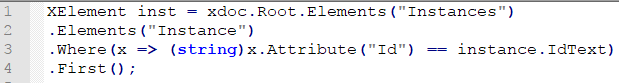
\includegraphics {linqprzyklad}
	\caption{Przykład wprowadzania instancji problemu układania planu zajęć za pomocą biblioteki \textit{Xml.Linq}.}
	\label{fig: linqprzyklad}
\end{figure}

Wprowadzone dane zapisywane są w bazie danych, dlatego każde kolejne wykonanie aplikacji umożliwia pracę na już wczytanych danych. Jak stwierdzono w poprzednich rozdziałach, założono, że wprowadzone dane zawierają zdarzenia z przypisanymi wcześniej zasobami, takimi jak nauczyciel, sala i grupa.


\section{Specyfikacja wewnętrzna programu}

Poprzedni podrozdział miał na celu przedstawienie pomysłu i sposobu w jaki zaimplementowany został algorytm wyszukiwania z tabu. Ten podrozdział zawiera szczegóły techniczne implementacji, opis użytych narzędzi, używanych klas oraz zawiera najistotniejsze fragmenty kodu.



\subsection{Opis klas i ważniejszych funkcji}

Aplikacja zapisana jest w kilku folderach. Każdy z folderów zawiera klasy realizujące odrębne funkcje aplikacji. Folder \textit{Code} zawiera klasy realizujące algorytm wyszukiwania.  W folderze \textit{Data} znajdują się klasy służące do translacji plików wejściowych XML na obiekty, i zapisywania nowo powstałych obiektów do bazy danych. Folder \textit{Model} zawiera klasy odwzorowujące obiekty znajdujące się w bazie danych. Znajdują się więc tu klasy takie jak \textit{Instance, Event, Resource}. Ostatni folder, \textit{ViewModel}, przechowuje klasy realizujące przygotowanie danych to zaprezentowania ich w interfejsie graficznym. Poza folderami znajduje się osobna klasa \textit{Form1}, która obsługuje interfejs graficzny użytkownika.

Poniżej przedstawiono ważniejsze klasy programu wraz z opisem funkcji w nich zawartych.

\begin{itemize}
	\item  \textit{Code/SolutionManager} - klasa zawiera szkielet algorytmu wyszukiwania z tabu. Jest to główna klasa algorytmu.  Znajdują się w niej funkcja rozwiązująca problem układania planu zajęć dla instancji o podanym identyfikatorze. Klasa ta zawiera również funkcje zapisującą raport działania algorytmu do pliku txt oraz funkcję wyświetlającą rozwiązanie na konsolę. Główna funkcja klasy zaprezentowana została na rysunku 6.2.
	
	\begin{figure}
	\centering
	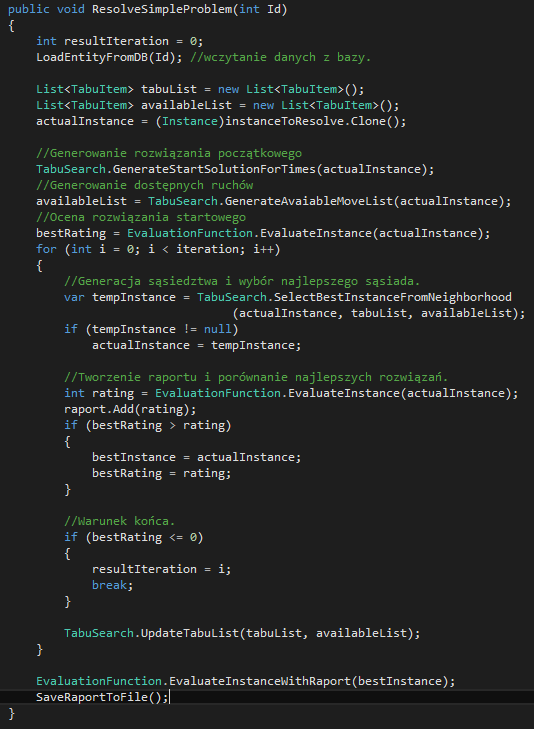
\includegraphics {ResolveSimpleProblem}
	\caption{Funkcja \textit{ResolveSimpleProblem} zawierająca szkielet algorytmu Tabu search. }
	\label{fig: ResolveSimpleProblem}
	\end{figure}

	\item \textit{Code/TabuSearch} - klasa zawiera statyczne funkcje służące do rozwiązywania problemu za pomocą algorytmu wyszukiwania z tabu. Znajdują się tu funkcję generujące dostępne ruchy, losowe rozwiązanie startowe, aktualizujące listę tabu, generujące sąsiedztwo i wybierające z nich najlepszego osobnika. W tej klasie znajdują się najważniejsze fragmenty kodu implementujące algorytm wyszukiwania z tabu. Funkcja generująca sąsiedztwo i wybierająca z niego najlepszą instancje została zaprezentowana na rysunku 6.3.

	\begin{figure}
	\centering
	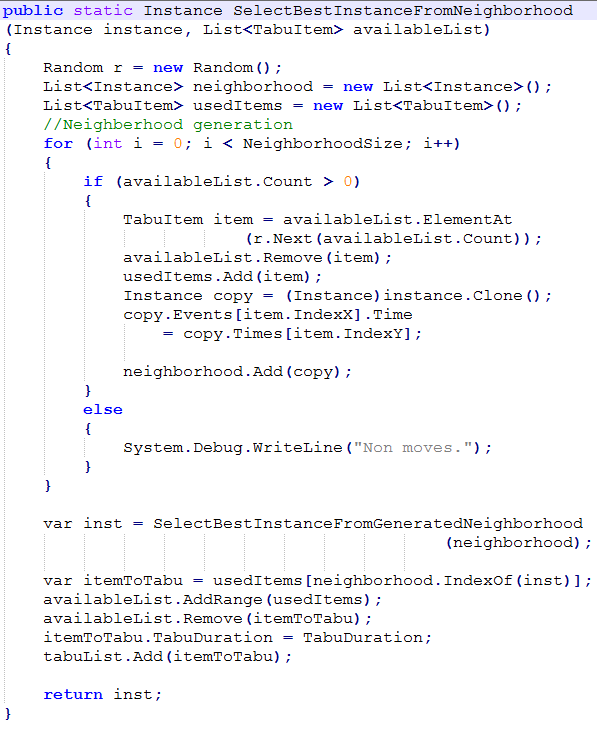
\includegraphics {SelectbestInstance}
	\caption{Funkcja \textit{SelectBestInstanceFromNeighborhood} generująca sąsiedztwo i wybierająca najlepszego sąsiada. }
	\label{fig: SelectbestInstance}
	\end{figure}

	\item \textit{Code/EvaluationFunction} -  w skład tej klasy wchodzą funkcje oceniające bieżące rozwiązanie uzyskane przez algorytm. Znajduje się tu implementacja wszystkich ograniczeń, jakie mają być uwzględnione w rozwiązaniu. Klasę tę można w łatwy sposób rozszerzyć dodając kolejne funkcje oceniające, które odpowiadają kolejnym ograniczeniom.
	 
	\item \textit{Code/TabuItem} - klasa reprezentująca pojedynczy ruch w algorytmie wyszukiwania z tabu. Jako ruch rozumiana jest para dwóch indeksów, pierwszy z nich odpowiada identyfikatorowi zdarzenia, a drugi to identyfikator okna czasowego, które w danym ruchu jest do tego zdarzenia przypisane.  Elementy klasy przechowywane są na liście tabu, dlatego klasa zawiera dodatkową właściwość, jaką jest czas trwania na liście tabu dla danego elementu.
	 
	\item  \textit{Data/XMLLoader} - w tej klasie zawarte są funkcje przekształcające dane wejściowe w formacie XHSTT, zapisane w języku XML, na klasy modelu. Znajduje się tu również funkcja zapisująca odczytaną instancje do bazy danych.
	
	\item \textit{Form1} - klasa obsługująca interfejs użytkownika. Zawiera funkcje reagujące na każdą wykonaną przez użytkownika czynność oraz funkcje wypisujące dane do odpowiednich obiektów interfejsu.
\end{itemize}

\section{Specyfikacja zewnętrzna programu}

	Po zainicjowaniu działania aplikacji wyświetlane jest okno główne przedstawione na rysunku 6.4. Przy pierwszym wykonaniu aplikacji użytkownik powinien wczytać instancje z pliku wejściowego. Może to wykonać za pomocą przycisku ,,Load instance from file'', który znajduje się w prawym górnym rogu okna. Otworzy się okno dialogowe, gdzie należy wskazać plik XML zawierający dane wejściowe dla problemu rozwiązywania planu zajęć, zapisane w formacie XHSTT. Po wczytaniu wielu instancji (lub po ponownym zainicjowaniu działania aplikacji), użytkownik może wybrać instancje do rozwiązania. Służy do tego rozwijana lista w lewym górnym rogu okna.
	
	Przycisk ,,Resolve'' służy do wykonania algorytmu. Działanie algorytmu jest monitorowane, a postępy wyświetlane są na konsoli na dole okna aplikacji. Po zakończeniu obliczeń, ułożony plan zajęć można oglądać w tabeli. Rozwijana lista nad tabelą służy do wyboru klasy, dla której ma zostać zaprezentowany plan zajęć.
	
	Użytkownik może zmieniać parametry algorytmu. Algorytm ma trzy parametry, których opis znajduje się poniżej:
	
	\begin{itemize}
		\item Iterations - maksymalna liczba iteracji jaką algorytm wykona w czasie rozwiązywania problemu układania planu zajęć. Jeżeli algorytm wcześniej znajdzie rozwiązanie, na które nie jest nałożona żadna kara, to zakończy swoje działanie.
		\item Tabu duration - parametr oznaczający czas pozostawania pojedynczego ruchu na liście tabu. Długość mierzona jest liczbą iteracji algorytmu.
		\item Neighborhood - rozmiar sąsiedztwa jakie zostanie losowo wybrane i przeszukane podczas jednej iteracji algorytmu. Rozmiar sąsiedztwa nie powinien być większy od liczby wszystkich dostępnych ruchów, które może wykonać algorytm (pełne sąsiedztwo).
	\end{itemize}
	
	\begin{figure}
	\centering
	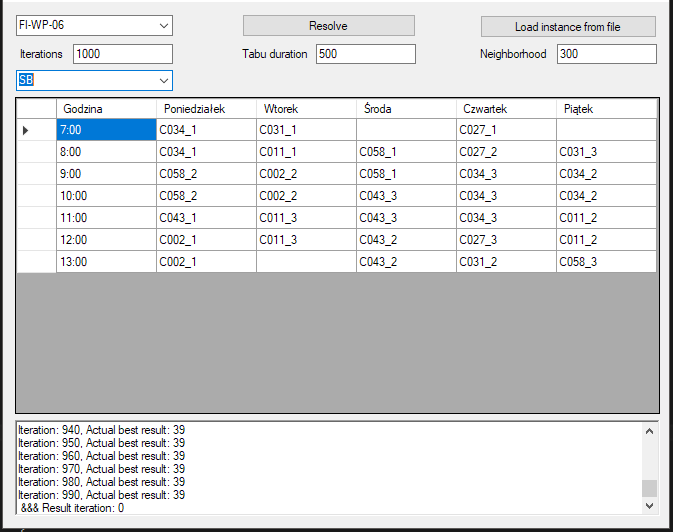
\includegraphics[width=\textwidth] {Aplikacja}
	\caption{Okno główne aplikacji.}
	\label{fig: Aplikacja}
	\end{figure}
\chapter{Testowanie aplikacji}

\section{Środowisko testowe}

Aplikacja została zrealizowana i testowana na komputerze stacjonarnym z systemem operacyjnym Windows 10. Wyposażenie komputera było następujące:

\begin{itemize}
\item procesor Intel Core i5-4670K 3.40 GHz,
\item karta graficzna Nvidia GeForce GTX 770,
\item pamięć operacyjna RAM 8 GB DDR3,
\item dysk twardy SSD Crucial CT120M.
\end{itemize}

\section{Zestaw danych testowych}

Jako zestaw danych testowych, z pomocą których testowany był algorytm układania planu zajęć, wybrany został zestaw fińskiej szkoły ponadpodstawowej. Oparty on został na danych z roku 2006 szkoły West-Pori High School, w której wiek uczniów należał do przedziału 16-19 lat. Zestaw został wybrany z uwagi na rozmiar danych oraz duże podobieństwo siatki zajęć do polskiego gimnazjum.

Wyżej wymieniony zestaw danych zawiera jedną instancję problemu układania planu zajęć. W instancji tej występuje:

\begin{itemize}
\item 35 okien czasowych rozłożonych na 5 dni w tygodniu (maksymalnie 7 zajęć dziennie),
\item 18 dostępnych nauczycieli,
\item 13 sal, w których mogą być prowadzone zajęcia,
\item 10 grup uczniów,
\item 172 wydarzenia o łącznej długości 297 okien czasowych (wiele zajęć dwu- i trzy-godzinnych).
\end{itemize}

Pokrycie okien czasowych w tym planie zajęć wynosi około 85\%. Liczba ta jest stosunkiem łącznego czasu trwania wydarzeń do całkowitej liczby dostępnych okien czasowych dla wszystkich grup (35x10). Analizując pokrycie można określić stopień trudności wykonania danego zadania układania planu zajęć. Dla pokrycia wynoszącego 100\% ułożenie poprawnego planu zajęć jest bardzo trudne, ponieważ w oczekiwanym planie zajęć nie może być ani jednego wolnego okna czasowego. Pokrycie wynoszące 85\% to średnio zaawansowany stopień trudności. Dla porównania, pokrycie planu zajęć dla polskiego liceum wynosi średnio 75\%.

Testowany zestaw danych wejściowych zawiera cztery ograniczenia:

\begin{itemize}
\item przypisany czas dla wszystkich zdarzeń,
\item unikanie konfliktów zasobów,
\item brak podziału zdarzeń,
\item ograniczenie bezczynności uczniów (okienek w planie).
\end{itemize}

Ograniczenia te zostały szczegółowo omówione w rozdziale 4.

\section{Wyniki działania aplikacji}

Aplikacja została wykonana wielokrotnie dla różnych parametrów. Średni czas pracy aplikacji wynosił ok. 8 minut. Najlepszy wynik, jaki udało się uzyskać to plan zajęć o ocenie 12. Oznacza to, że w otrzymanym planie zajęć nie wystąpił żaden konflikt zasobów, oraz że wystąpiło tylko 6 okienek (wolnych okien czasowych między zajęciami), co daje wynik około jednego okienka na dwie klasy uczniów. Jest to wynik bardzo dobry. Na rysunkach 7.1 i 7.2 przedstawiono najlepszy i najgorszy plan dla różnych klas uczniowskich w tym rozwiązaniu. Kolory ilustrują zajęcia o czasie trwania większym niż jedno okno czasowe.

\begin{figure}
	\centering
	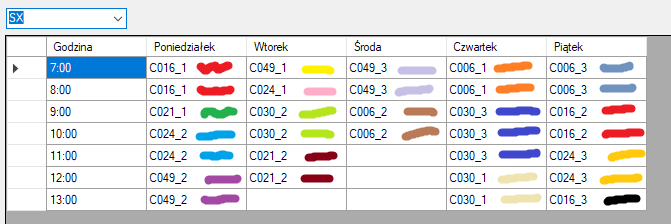
\includegraphics[width=\textwidth] {sx}
	\caption{Najlepszy otrzymany plan zajęć spośród planów dla dziesięciu klas.}
	\label{fig: sxkopia}
	\end{figure}
	
	\begin{figure}
	\centering
	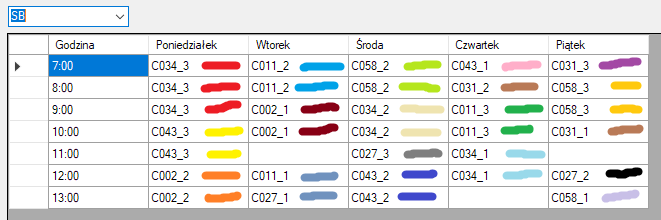
\includegraphics[width=\textwidth] {sb}
	\caption{Najgorszy otrzymany plan zajęć spośród planów dla dziesięciu klas (dwa okienka).}
	\label{fig: sbkopia}
	\end{figure}

Wykres na rysunku 7.3 przedstawia drogę algorytmu jaką musiał pokonać w czasie swojej pracy. Na osi pionowej przedstawiona jest  ocena aktualnego rozwiązania a  na osi poziomej liczba iteracji.

	\begin{figure}
	\centering
	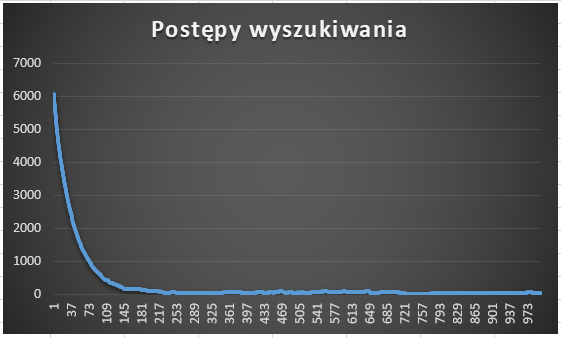
\includegraphics[width=\textwidth] {postepywyszukiwania}
	\caption{Przebieg pracy algorytmu.}
	\label{fig: postepywyszukiwania}
\end{figure}

Najlepszy wynik otrzymany został dla następujących parametrów algorytmu: liczba iteracji - 1000, czas trwania tabu - 500, rozmiar sąsiedztwa  - 300. Liczba iteracji algorytmu została ustalona, biorąc pod uwagę czas pracy programu oraz to, że liczba ta zazwyczaj wystarczała, by usunąć wszystkie konflikty z planu zajęć. 

Rozmiar sąsiedztwa również w dużej mierze wpływa na czas pracy algorytmu. Doświadczenia pokazały, że im większe sąsiedztwo tym mniej iteracji potrzebnych jest do uzyskania lepszych wyników. Rozmiar 300 to około 5\% całego sąsiedztwa możliwego do przeszukania. Przyjęcie rozmiaru sąsiedztwa na 100\%, spowodowało by wydłużenie pracy algorytmu dwudziestokrotnie. Ustalony rozmiar jest próbą pogodzenia oczekiwań, jak najkrótszego czasu pracy algorytmu i jak najlpeszych wyników.

Czas trwania tabu zmienia całkowicie sposób pracy algorytmu. Ustalenie wartości 500 wynikało z obserwacji wyników, jakie uzyskał algorytm oraz wykresów obrazujących jego pracę. Szczegółowe omówienie wpływu parametru czasu trwania tabu przedstawiono w kolejnym podrozdziale.

\section{Wpływ czasu trwania tabu na uzyskane wyniki.}

Algorytm wyszukiwania z tabu opiera się na algorytmie przeszukiwania lokalnego, w który stosuje się listę tabu. Parametr określający czas pozostawania ruchów na liście tabu ma duże znaczenie. Zmiana tego parametru powoduje zupełnie inną pracę algorytmu. Potwierdzeniem tego są wykresy przedstawione na rysunkach 7.4 - 7.8.

Na wykresach przedstawiono przebieg pracy algorytmu dla parametrów: 1000 iteracji i rozmiar sąsiedztwa równy 300. Zmieniał się tylko parametr długości tabu. Jak można zauważyć na rysunku 7.3, algorytm w początkowej fazie pracy znacznie poprawia swój wyniki (zmniejsza ocenę rozwiązania z 6000 do ok. 200). Z tego powodu na analizowanych obecnie wykresach przedstawiono tylko ostatnie 800 iteracji pracy algorytmu, by obciąć początkowy ,,skok'' i móc zaobserwować zmiany pracy algorytmu w mniejszej skali.

\begin{figure}
	\centering
	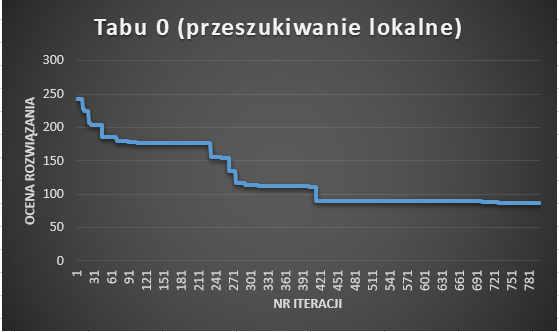
\includegraphics[width=\textwidth] {0}
	\caption{Przebieg pracy algorytmu dla czasu trwania tabu = 0.}
	\label{fig: 0}
\end{figure}

\begin{figure}
	\centering
	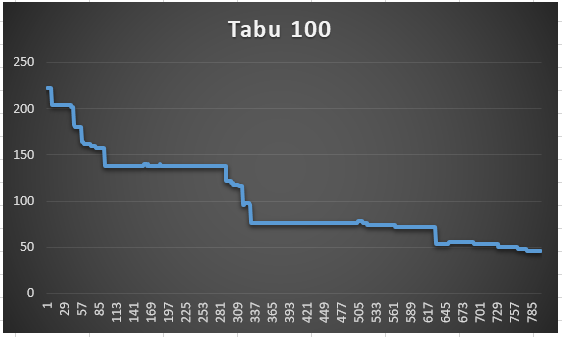
\includegraphics[width=\textwidth] {100}
	\caption{Przebieg pracy algorytmu dla czasu trwania tabu = 100.}
	\label{fig: 100}
\end{figure}

\begin{figure}
	\centering
	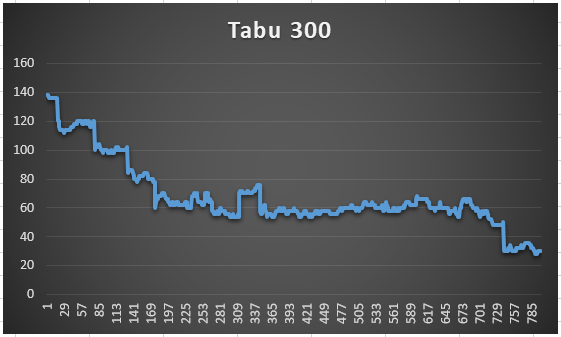
\includegraphics[width=\textwidth] {300}
	\caption{Przebieg pracy algorytmu dla czasu trwania tabu = 300.}
	\label{fig: 300}
\end{figure}

\begin{figure}
	\centering
	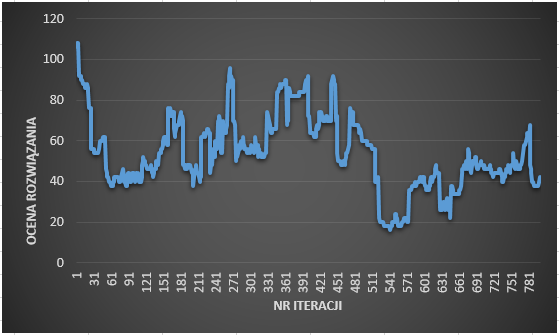
\includegraphics[width=\textwidth] {500}
	\caption{Przebieg pracy algorytmu dla czasu trwania tabu = 500.}
	\label{fig: 500}
\end{figure}

\begin{figure}
	\centering
	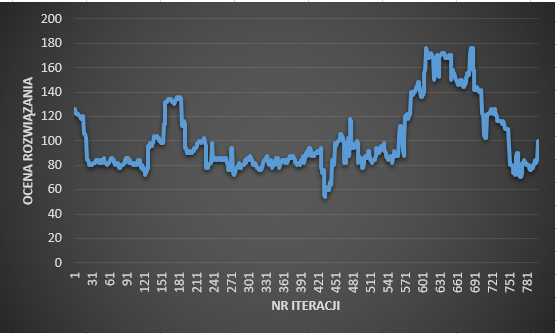
\includegraphics[width=\textwidth] {800}
	\caption{Przebieg pracy algorytmu dla czasu trwania tabu = 800.}
	\label{fig: 800}
\end{figure}

Pierwszy z wykresów (rysunek 7.4) prezentuje pracę algorytmu dla długości tabu równej 0. Oznacza to, że algorytm w ogóle nie korzysta z listy tabu. Jest to więc klasyczne przeszukiwanie lokalne. Jak widać, algorytm przeszukuje rozwiązania, które mają tą samą ocenę lub wyższą. Na wykresie nie można zauważyć skoku oceny wartości ,,w górę''. Jest to spowodowane wpadaniem algorytmu w lokalne minima, a poprawa rezultatu najczęściej jest skutkiem innego losowego wyboru sąsiadów. ocena planu jaką udało się osiągnąć to 84.

Drugi wykres (rysunek 7.5) przedstawia przebieg pracy algorytmu dla długości tabu równej 100. Otrzymany wykres jest bardzo zbliżony do poprzedniego, jednak można zaobserwować nieliczne próby pogorszenia oceny rozwiązania bierzącego w celu dotarcia do rozwiązania lepszego. Najlepszą uzyskaną oceną rozwiązania była ocena 48. Jak widać, 100 ruchów zabronionych z puli 6000 dostępnych (dla tego przypadku testowego), to zdecydowanie za mało, by efektywnie korzystać z zalet wyszukiwania z tabu.

Na trzecim wykresie (rysunek 7.6) sytuacja wygląda już zdecydowanie lepiej. Długość tabu równa 300 sprawia, że algorytm przeszukuje obszary, do których można dotrzeć tylko przez pogorszenie bieżącego wyniku. Większe skoki oceny rozwiązań to miejsca, w których udało się wyeliminować konflikt zasobów (każdy konflikt nakłada karę 20). Mniejsze zmiany obrazują próby minimalizacji okienek (każde okno czasowo powiększa ocenę rozwiązania o 2). Najlepszy uzyskany wynik to 30.

Czwarty wykres (rysunek 7.7) prezentuje sytuację, w której udało się osiągnąć najlepsze rezultaty (w tym przypadku oceną 18 - rozwiązanie optymalne to ocena 0). Najlepszy wynik udało się osiągnąć już w 740 iteracjach (540 plus 200 iteracji nie przedstawionych na wykresie). Dla długości listy tabu równej 500 przeszukiwanie odbywa się już bardzo ,,skokowo''. Algorytm nie może wykonać 500 ruchów, które w poprzednich iteracjach najbardziej poprawiły wyniki algorytmu. Musi jako bieżące rozwiązanie przyjąć rozwiązanie o gorszej ocenie. Dzięki temu jest w stanie dotrzeć do obszarów, które dla przeszukiwania lokalnego są nieosiągalne.

Ostatni wykres (rysunek. 7.8) przedstawia przebieg algorytmu dla długości tabu równej 800. Przy 1000 iteracjach tylko pierwsze 200 ruchów mogło zostać powtórzone. Niestety, tak duża liczba zabronionych ruchów spowodowała, że algorytm zdecydowanie pogorszył swoje wyniki (najlepszy rezultat to ocena 52). Choć algorytm próbował przejść w inne obszary poszukiwań, to nie otrzymano oczekiwanych rezultatów. Najprawdopodobniej, kluczowe ruchy znajdowały się na liście tabu.

\begin{figure}
	\centering
	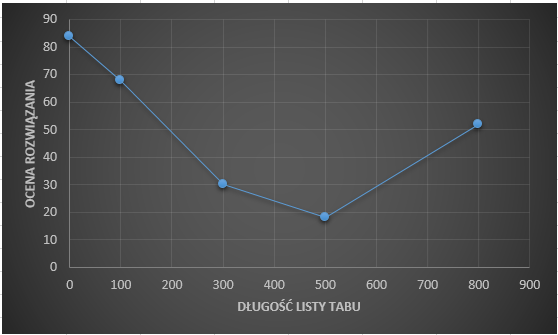
\includegraphics[width=\textwidth] {ocenadodlugosci}
	\caption{Stosunek długości listy tabu do uzyskanej oceny rozwiązania - wykres.}
	\label{fig: ocenadodlugosci}
\end{figure}

\begin{figure}
	\centering
	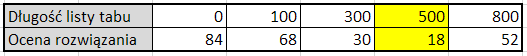
\includegraphics[width=\textwidth] {tabelaocen}
	\caption{Stosunek długości listy tabu do uzyskanej oceny rozwiązania - tabela.}
	\label{fig: tabelaocen}
\end{figure}

Rysunek 7.9 i 7.10 przedstawiają stosunek parametru długości listy tabu do otrzymanego rozwiązania. Najlepszy rezultat otrzymano dla parametru długości listy tabu równego 500. Ocena rozwiązania optymalnego, którą algorytm starał się osiągnąć jest równa 0.
\chapter{Podsumowanie}

Głównym celem niniejszej pracy było zastosowanie algorytmu przeszukiwania z tabu do rozwiązywania problemu układania planu zajęć. Cel ten został zrealizowany. Efektem pracy jest aplikacja, za pomocą której można ułożyć plan zajęć dla sformułowanego problemu zapisanego w formacie XHSTT. W aplikacji zaimplementowano cztery ograniczenia planu zajęć spośród dużej liczby dostępnych ograniczeń w formacie XHSTT. Pozostałe ograniczenia nie zostały zaimplementowane z powodu rzadkiego występowania w różnych danych testowych oraz ograniczeń czasowych wykonania niniejszej pracy. 

Podczas implementacji algorytmu, autor napotkał wiele trudności. Wszystkie z nich zostały pokonane. Pierwszą z nich było zapoznanie się z formatem danych wejściowych XHSTT, który mimo bardzo dobrej dokumentacji jest formatem stosunkowo złożonym i sprawia, że na problem rozwiązywania planu zajęć należy spojrzeć z innej strony. Kolejną trudnością była implementacja algorytmu ze względu na rozmiar danych wejściowych. Rozmiar ten był bardzo duży i trudno było zweryfikować poprawność pracy algorytmu. Dlatego zdecydowano się rozpocząć implementację, testując jej działanie na danych nierzeczywistych zawierających bardzo małą liczbę zdarzeń i zasobów. Podczas testowania pojawiła się trudność związana z długim czasem oczekiwania na wyniki oraz obiektywnym porównaniem jakości rozwiązań. Zdecydowano, aby generować raporty z pracy algorytmu w celu analizy jego działania w zależności od parametrów wejściowych.

Aspektem badawczym pracy była analiza pracy algorytmu dla różnych wartości długości tabu. W wyniku przeprowadzonej analizy pokazano, że najlepsze rezultaty algorytm osiągał dla listy tabu długości 4-5\% liczby wszystkich dostępnych ruchów. Czas pracy algorytmu zależny jest od rozmiaru danych wejściowych oraz od przyjętych wartości parametrów. Dla problemu układania planu zajęć dla szkoły o rozmiarze polskiego liceum o średniej wielkości oraz optymalnie dobranych parametrach, czas pracy algorytmu wynosi około 10 minut.

Zaimplementowany algorytm nadaje się do praktycznego użytkowania i może być wykorzystany dla większości problemów układania planu zajęć zapisanych w formacie XHSTT.

Możliwy jest dalszy rozwój aplikacji w postaci implementacji kolejnych ograniczeń oraz implementacji poprawnego zachowania algorytmu dla zajęć o długości dłuższej niż trzy okna czasowe. Osiągnięte rezultaty są satysfakcjonujące, jednak można poczynić starania, aby poprawić algorytm przeszukiwania przez dodanie metod dywersyfikacji i intensyfikacji do opracowanego algorytmu. Należy się jednak liczyć z tym, że każde dodatkowe ograniczenie wydłuży czas działania algorytmu, konieczna więc będzie jego optymalizacja.



%   this is for BibTeX.  remove if you plan to write the references in the document
%\bibliographystyle{plplain}
\bibliographystyle{plain}
\bibliography{refs}

%adds the bibliography to the table of contents
\addcontentsline{toc}{chapter}
         {\protect\numberline{Bibliografia\hspace{-96pt}}}
         
%dodatki
%\appendix
%\chapter{Symbole przyjęte w pracy}
\label{app:symbole}

Jeśli w tekście nie wykazano inaczej, stosowane symbole należy rozumieć jako:

\begin{itemize}
\item[$f(x,y)$] - jasność piksela o współrzędnych $(x,y)$ w obrazie wejściowym,
\item[$g(x,y)$] - jasność piksela o współrzędnych $(x,y)$ w obrazie wynikowym,
\item[$t$, $t_i$] - wartości progowe,
\item[$G$] - liczba poziomów szarości obrazu; $G=256$,
\item[$P(i,j)$] - macierz GLCM,
\item[$M(i,j)$] - maska przetwarzania.
\end{itemize}


%%%%%%%%%%%%%%%%%%%%%%%%%%%%%%%%%%%%%%%%%%%%%%%%%%%%%%%%
\chapter{Inny, przykładowy dodatek}
\label{app:dodatekPrzyklad}

\end{document}